\chapter{Framework for Comparing Time Series Classification Algorithms in Early Classification Context}
\label{ChapterFramework}
This chapter describes our proposed framework which compares TSCAs in a context that is inspired by the problem of eTSC.
We begin by defining what we mean by early classification context and how our framework design simulate such context for TSCAs to operate in.
Then we discuss the conceptual structure of the framework, our implementation for its different components and how to evaluate it.
In this chapter we will be answering our research questions:
\begin{itemize}
  \item How to adapt existing TSC workflows for the early TSC context ?
  \item How to evaluate classifiers in the early TSC context ?
  \item How to evaluate the proposed solution ?
\end{itemize}


\section{Early Classification Context}
\label{SectionEarlyClassificationContext}
%% Intro
As motivated earlier, eTSC is a field which is concerned with classification of time series data with earliness and accuracy
as the main objectives. Dedicated eTSCAs focus on building models that can learn class labels of the data as early as possible
while maintaining accuracy \cite{mori2017early}.
Our framework, on the other hand, investigates the adaptation of the context in which conventional TSCA operate to learn a specific
classification problem and the effect it has on the classifiers' performance.

We define our early classification context as the problem in which a conventional TSCA is trained on labeled but incomplete time series data.
Then this trained model is used to classify unseen data instances of full length.
This context helps investigate if TSCA are able to learn about the problem at hand without having to wait for the full data to be made available.
In other words, the benefit acquired from waiting for more data points to be made available for learning is less than the benefit of having a slightly less accurate result but at an earlier point of time.

\section{Conceptual Design}
\label{SectionConceptualDesign}
To answer our first research question \textbf{\textit{How can we adapt existing TS classification workflow for the early TS scenario ?}}
We propose a framework that simulates an early classification context by shortening the length of the data before feeding it to TSCAs to learn on.
These classifiers are then evaluated by comparing their performance to a baseline represented by their performance on the full length data.
In the beginning, the framework divides whole timeseries data instances into smaller subsequences using a chopping algorithm, and then starts multiple learning processes.

For the first learning process, it feeds only one subsequence for the classifier to learn on.
Then in each following learning process, the framework adds the next subseuqnce to the training data in addition to the previous ones.
These processess simulate an incremental learning scenario, where the classifier is not exposed to all the data points collected from the beginning to the end at once, but rather exposed to the data in a sequential procedure.
During each learning process the classifier gets to learn more information about the data instances than the previous process.
Finally, to assess how good the performance of the classifiers that were exposed to less data points is, we compare their performance to that of a baseline.
The baseline for each classifier is determined by its performance when exposed to full length training data.

Our framework design can be divided into two main components; the comparison testbed and the recommender.
Each of these components consists of smaller elements which are responsible for specialized tasks which we will discuss in more details.
Figure \ref{Img:ConceptualDesign} shows the conceptual design of the framework and all its costituent components.

\begin{figure}[!htbp]
  \captionsetup{justification=raggedright}
  \centering
  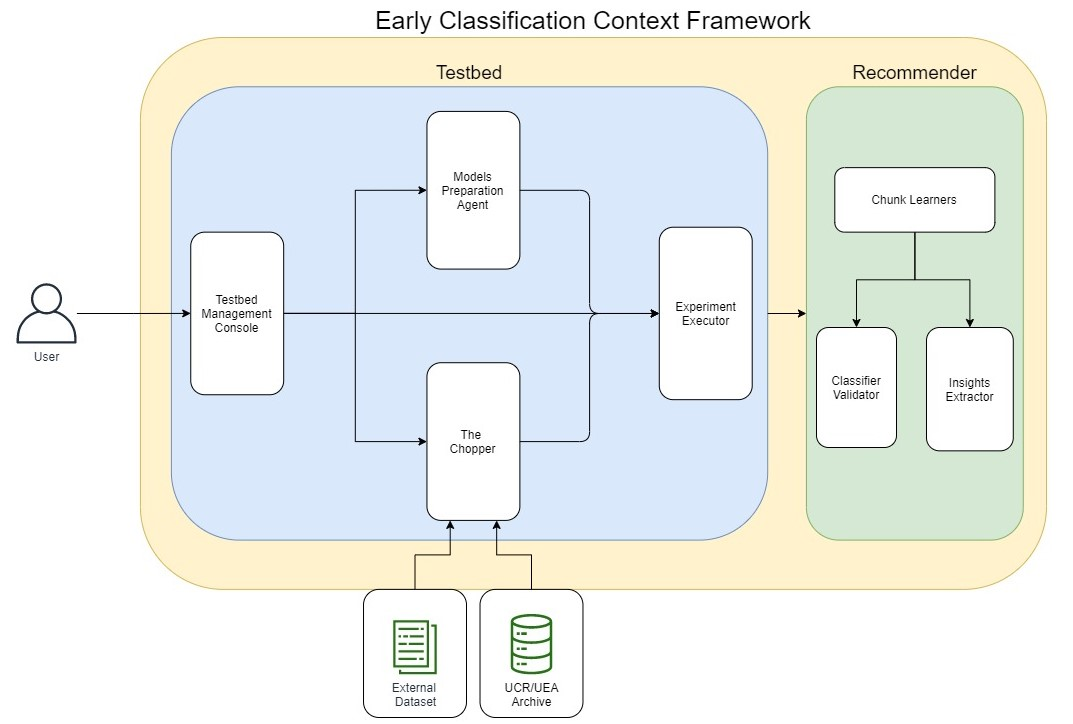
\includegraphics[width=\textwidth]{Framework Diagram.jpg}
  \centering
  \caption{Conceptual design of the proposed framework}
  \label{Img:ConceptualDesign}
\end{figure}

\subsection{The Testbed}
\label{SubsectionTestbed}
The first component is the comparison testbed. It is the main engine of the framework for configuring and executing learning processes.
There are multiple units that make up the testbed. These are; the testbed management console, the model preparation agent, the chopper and the experiment executor.
Each of these units is responsible for a specific task and communicate information either to the other units in the testbed or to other units in the recommender.

\subsubsection*{The Testbed Management Console}
\label{TestbedManagementConsole}
In order for the testbed to be able to configure its components and experiments, it needs to collect information about the desired shape of experiments.
The testbed management console is the interface which the user interacts with to provide all the necessary information.
The console allows the user to specify details about the data sets to be used, the configuration of the chopping algorithm
and the struture of the experiments to be executed in terms of models specification, training and testing processes design.
The testbed management console creates the central configuration which will be followed by all the other elements.

\subsubsection*{The Model Preparation Agent}
\label{ModelPreparationAgent}
The model preparation agent is responsible for constructing and composing the classification models that will be used in the learning processes.
Based on the configuration from the testbed management console, the model preparation agent includes or excludes models from the experiments
and supply the hyperparameter space for each model. The configured models are then passed to the experiment executor.

\subsubsection*{The Chopper}
\label{Chopper}
The chopper algorithm is the essence of the early classification context. It is the component which simulates the incremental learning scenario for the classifiers.
Based on the configuration from the testbed, the chopper collects information about the different data sets that will be used in the learning processes.
Then for each data set, it applies the chopping on its data instances based on their length.
The chopped data would then be combined with the algorithm; to start the learning processes.

\subsubsection*{The Experiment Executor}
\label{ExperimentExecutor}
The last element in the testbed is the experiment executor.
It collects the configured models from the model preparation agent along with the chopped data sets from the chopper for the actual execution of the experiments.
Based on the central configuration, it configures the environment for the learning proccesses to provide unbiased results, as well as sets the evaluation scheme of the testing process.
After the experiments are finished, it provides insights from the results for each process.
It also communicates the results and analysis for the recommender to learn on.

\subsection{The Recommender}
\label{SubsectionRecommender}
The other component of the framework is the recommender.
As the name suggests, the recommender is responsible for providing reliable suggestions about the most suitable classifiers to use for unseen data sets.
Based on results from the testbed experiments, it learns to predict the performance of different classifiers on data sets in the early classification context.
Then when provided with an unseen data set, the recommender would suggest which classifier or multiple classifiers will attain good results if used to learn
on incomplete subsequences of data. The recommender consists of three elements; the chunk learners, the classifier validator and the insights extractor.

\subsubsection*{The Chunk Learners}
\label{ChunkLearners}
The chunk learners are a group of classifiers which learn on the results from the experiments of the testbed.
The word chunk in the name refers to the chunks (subsequences) that were shown for the classifiers to learn on.
Each learner is responsible for learning on the performance of classifiers for a given chunk and consequently predicting the performance of these classifiers for unseen data sets.
The prediction results are then passed to the classifier validator and the insights extractor.

\subsubsection*{The Classifier Validator}
\label{ClassifierValidator}
The classifier validator is a component which assesses the prediction results from the chunk learners.
Its main objective is to decide if the predicted performance results for the classifiers on a data set qualify as good recommendations or not.
The classifier validator should exclude classifiers from the recommendations if it evaluates their performances as weak and not competent.
The result from the classifier validator is the actual final recommendations of the framework.

\subsubsection*{The Insights Extractor}
\label{InsightsExtractor}
The insights extractor is responsible for analyzing and extracting insights from the results of the chunk learners.
It reveals hidden patterns and provides understandable insights about how the performance predictions were made
and how recommendations were chosen.

\section{Implementation}
\label{SectionImplementation}
This section describes our implementation for the framework and all of its components.
In the beginning we discuss our design protocol for building the framework.
Then we demonstrate our technical design for each of the components, the selected toolkits for building the components
and the flow of information through communication channels that exist between the framework's units.

\subsection{Design Protocol}
\label{SubsectionProtocol}
Our design protocol covers the main design aspects in the framework like; the selection criteria of the classifiers to be included
and the evaluation criteria for assessing the performance of the classifiers.

There is a wide variety of TSCAs that has been introduced in the last decade.
Since our goal is to compare TSCAs in the early classification context, we specify an inclusion criteria which would cover this wide spectrum of classifiers.
To represent the currently available techniques; we follow the grouping criteria mentioned in \cite{bagnall2017great} that breaks down classifiers into 5 main groups based on the technique applied.
In addition to a \nth{6} group which represents deep learning TSCAs. We represent each of the groups by 2 classifiers; one which is an ensemble and another which is a non-ensemble.
The reason we include both ensembles and individual classifiers; is that although for each group there is a classifier which can outperform the others,
yet combining classifiers in an ensemble have proven to outperform all of its individual classifiers \cite{fawaz2019deepreview}.

The other aspect of the framework is to choose an evaluation criteria for assessing the performance of classifiers.
Since our framework is inspired by the problem of eTSC; we are interested in evaluating classifiers based on their performance in predicting correct class labels, as well as considering how early they make the prediction.
Previous eTSC research have used the harmonic mean of accuracy and earliness as an evaluator for classifiers \cite{schafer2020teaser}; because it allows combining both in a single score.
The harmonic mean considers both earliness and accuracy to be equally important.
In our framework we use $F_{\beta}$; a generalized form of the harmonic mean which allows the assignment of different weights to earliness and accuracy using the parameter $\beta$.
We prefer using $F_{\beta}$ to offer more flexibility in adjusting weights to suit cases where either of the objectives is more important than the other.

We also use a baseline classifier, which is a non-time series classification algorithm.
It is a simple classifier which always predicts the majority class of a given data set.
We include this classifier not as a competing algorithm, but as a basic standard; to better understand the actual performance of the other classifiers on the data sets and assess the quality of their results.
We use the results from this baseline classifier in the testbed and the recommender; as a threshold that we can compare other classifiers to and define a notion of goodness and badness for performance.
We name the classifier \emph{dummy}; as an indication of its role in the comparisons and will refer to it using that name.

%The testbed is the engine responsible for comparing the implemented algorithms on the data sets provided.
%The testbed mainly collects user input about the experiment configuration, preprocesses the data in preparation for the learning process
%and finally calculates performance metrics using testing data.
%By the end of each performance assessment step, the testbed produces an analysis file and a logs file.
%The logs file provides information about the setup of the experiment, the execution status, the duration and reasons of failure.
%While the analysis file provides information about the cross validation scorese, the final hyperparameter values used, processing time of training and testing steps and the performance measures.

%The second step of the framework is learning a recommender which will be able to predict the best performing algorithm(s) for an unseen data set.
%Given the different analysis reports generated from the testbed, these reports are then consolidated and fed to the recommender to learn on.
%First, the logging files are processed and filtered to get the data of the successfully executed processes.
%Then the analysis files for these proccesses are consolidated into a unified structure and the included information is enriched by metadata about the data sets.
%In the end, the data is preprocessed again to be fed to a regression classifier which learns from the results of already carried out experiments.
%When given a new data set, the regression classifier tries to predict the performance of each implemeted classifier on the data set.
%These scores are then used to rank the classifiers and the final recommendation is presented.


\subsection{Toolkits}
\label{SubsectionToolkits}
% Libraires we use
We implemented our framework in python language.
For the implementation of the non-deep learning algorithms we used the open source libraires $sktime V. 0.5.3$ \cite{loning2019sktime} and $pyts V. 0.11.0$ \cite{JMLR:v21:19-763},
while for the implementation of the deep learning algorithm InceptionTime we used the library $sktime\-dl V .0.2.0$ which provides an interface for the implementation provided
in the study \cite{fawaz2020inceptiontime}. Finally, we used the library $Tslearn V. 0.5.0.5$ \cite{JMLR:v21:20-091} as a mediator between the different model implementations; due to its
capacity to process raw data into the needed input format by any of the libraries, as well as converting data format between the different libraires.

\subsection{The Testbed Implementation}
\label{SubsectionTestbedImplementation}

\subsubsection{The Testbed Management Console Implementation}
\label{SubsectionTestbedManagementConsoleImplementation}
% User Input
The Testbed Management Console is the tool that allows the user to interact with the framework and configure the experiments
and the learning processes which will be the basis of the final recommendations.
At this stage, the user provides the necessary information required by the framework to formulate and start its learning experiments.
These information provide the guidelines for the other components in the framework like the model preparation agent and the data chopper.
Which are essential for the preparation of data sets and models for the learning processes.
Table \ref{TableUserInput} shows a summary of each of the needed information, represented as a parameter for the framework.

\begin{table}[hbt!]
  \setlength\extrarowheight{2pt} % for a bit of visual "breathing space"
  \begin{tabularx}{\textwidth}{|X|X|X|}
  \hline
  \textbf{Parameter} & \textbf{Data Type} & \textbf{Description} \\ \hline
    Dataset         & String List        & The name of the data set(s)                        \\ \hline
    Splits          & Integer            & The number of splits to apply on the data set      \\ \hline
    Hyperparam      & Boolean            & Learn hyperparameters for the model or skip        \\ \hline
    NumIterations   & Integer            & Number of hyperparameters combinations to sample   \\ \hline
    ChunksToKeep    & Integer List       & The indexes of the chunks to use                   \\ \hline
    FromBeg         & Boolean            & Reveal data chunks from beginning or end           \\ \hline
    ScoringFunction & String             & The strategy for evaluating the model on test data \\ \hline \\
  \end{tabularx}
  \caption{Input parameters required for using the framework}
  \label{TableUserInput}
\end{table}

We implemented the user input interface using $docopt$ \footnote{https://github.com/docopt/}. A library which offers command-line interfaces through
the use of simple arguments and elements. It also allows setting default values for parameters which can be overriden if a value is passed.
To start running the framework, one provides the necessary parameter values through a simple terminal command.
Listing \ref{ListingUserInput} shows a sample command for running our master python file $run.py$ on the Computers data set using hyperparameters optimization,
while applying a split into 10 chunks.

\lstset{basicstyle=\ttfamily\small}
\begin{lstlisting}[language=Comsol,caption={Sample command for providing user input to the framework},captionpos=b,label={ListingUserInput}]
  python run.py --etsc --dataset=Computers --cv --split=10
\end{lstlisting}

\subsubsection*{The Model Preparation Agent Implementation}
\label{ModelPreparationAgentImplementation}
The model preparation agent is responsible for preparing the time series classifers and creating their hyperparameter space for each learning process.
We design our model preparation agent to adjust the preparation of models to handle univariate and multivariate data sets.

As mentioned in section \ref{SectionTSCA}, we follow the grouping criteria by \cite{bagnall2017great} which arranges TSCAs into 5 main categories based on their techniques.
We have included classifiers representing each of the 5 groups, in addition to a \nth{6} group which represents the family of deep learning time series algorithms.
For each group, we have selected the state of the art classifier based on the results of previous comparison frameworks discussed in chapter \ref{ChapterRelatedWork}.
We tried, as far as the implemented libraries allowed, to represent each group with 2 classifiers; one that is a non-ensemble and another which is an ensemble.
A total of 10 classifiers are included in the framework covering all 6 groups, these can be broken down into the following:
\begin{itemize}
  \item Distance based : 1NN using MSM distance and PForest
  \item Phase dependent algorithms : TSF
  \item Shapelets: LS and ST
  \item Dictionary based : WEASEL and BOSS
  \item Deep learning : InceptionTime
  \item Classical baselines: 1NN using euclidean distance and 1NN using DTW
\end{itemize}

Table \ref{TableClassifierParams} shows the configuration and hyperparameters for all the included classifiers.
We used the same hyperparameter space like that of the original published papers as closely as possible.

\begin{table}[hbt!]
  \setlength\extrarowheight{2pt} % for a bit of visual "breathing space"
  \begin{tabularx}{\textwidth}{|X|X|}
  \hline
  \textbf{Classifier} & \textbf{Parameters} \\ \hline
  MSM                 & c = \{0.01, 0.1, 1, 10, 100\}                                                        \\ \hline
  PForest             & k = 100 \newline r = 5                                                               \\ \hline
  TSF                 & r = 500 \newline splitting = \{entropy, gini\} \newline maxfeatures = \{sqrt, log2\} \\ \hline
  LS                  & $\lambda_{w}$ = \{0.01, 0.1, 1\} \newline
                        $L_{min}$ = \{0.025, 0.075, 0.125, 0.175, 0.2\} \newline R = \{1, 2, 3\} \newline
                        K = \{0.05, 0.15, 0.3\} \newline $\eta$ = 0.01 \newline
                        maxIter = \{2000, 5000, 10000\}                                                      \\ \hline
  ST                  & t = 60 mins \newline n=\{500,100\}                                                   \\ \hline
  CBOSS               & t = 60 mins \newline k=\{50, 100, 250, 500\} \newline s=250 \newline p=[0.5 - 1]     \\ \hline
  WEASEL              & ANOVA = \{True, False\} \newline bigrams =\{True, False\}
                        \newline binning = \{equi-depth, equi-width, information-gain\}                      \\ \hline
  Inception           & epochs = 1500 \newline batch size = 64 \newline $\eta$ = 0.001 \newline
                        kernel sizes = \{10, 20, 40\}                                                        \\ \hline
  DTW                 & full warping window                                                                  \\ \hline
  \end{tabularx}
  \caption{Parameters and configuration for TSCAs}
  \label{TableClassifierParams}
\end{table}

%Multivariate (models initialization)
As mentioned earlier in section \ref{GreatBakeoffMultivariate}, there are two ways to work on multivariate time series data sets \cite{ruiz2020great}.
The first way is by using bespoke multivariate classifiers which can deal with the multiple dimensions available in the data.
While the other is by using ensembles of univariate classifiers, each fit to a separate dimension under the assumption of independence between the dimensions.
Our framework applies the second technique for handling multivariate data sets.

The model preparation agent checks the metadata of the data sets that the management console communicated, then it determines the number of dimensions each data set comprises.
If the data set is univariate then the model preparation agent initalizes the default classifer implementations provided by the libraries.
In case the data set was found to be multivariate, it initializes a special classifier type which extends the usage of univariate classifiers for multivariate problems.
This special classifier is reffered to as $ColumnEnsembleClassifier$ in the $sktime$ library implementation and as the $MultivariateClassifier$ in $pyts$.

There are two assumptions that we make at this step in our framework.
First, we assume that to extend a specific univariate classifier to a problem, we should fit the same type of the classifer on all dimensions of the data.
This goes back to our goal, that we want to compare classifiers from different groups and not to create an ensemble which makes use of different classifiers
applying different techniques, like HIVE-COTE does.
Second, we assume that we always have to fit one classifier per dimension, which have proved to be not a feasible solution for high dimensional data sets.
We will discuss this in more details in our results.

After the model preparation agent finishes, it passes the initialized models to the experiment executor for the learning processes to actually start.


\subsubsection*{The Chopper Implementation}
\label{ChopperImplementation}
% Input Datasets
The chopper is the data sets handling module of the framework.
It is not only designed to apply chopping of the data based on the configuration, but also to load the data sets and preprocess it.
The chopper collects information about the data sets to be used, the number of splits (chops) to be applied, the chopping direction and the chops filteration.
These information are passed from the management console in the form of the parameters $Dataset$, $Splits$, $FromBeg$ and $ChunksToKeep$ respectively.

The first task of the chopper is to process input data.
It is configured to process data sets in either of two ways; automatic download from the UCR/UEA data archives,
or manually provided data sets that comply with some specifications.
Since the data loading module from $pyts$ \cite{JMLR:v21:19-763} offers integrated tools with the UCR/UEA data archives for fetching and downloading data,
we have configured our chopper to extend $pyts$ by transparently checking both data archives when provided with a data set name.
The other option would be to provide a data set folder holding the name of the data set.
Inside the folder there should exist one training data set file with the name \enquote{FolderName\_TRAIN} and one testing data set file with the name \enquote{FolderName\_TEST}.
Which is the case for most of the data sets from both archives.
For multivariate data sets, the chopper assumes that the training data set file, as well as the testing data set file, contains data of all dimensions.
For maximum compatibility, the chopper extends the data processing utilities from $sktime$ \cite{loning2019sktime}
which can read data sets that comply with the guidelines provided by the UCR and the UEA archives.
We consider \enquote{arff} format as the primary expected data type.

% Chopping Algorithm
Based on the assumption that all data instances are of the same length, we implement our early classification context using a time series chopping algorithm.
The algorithm is provided with some time series data set $T$ with instances of length $L$ and three user defined parameters.
Parameter $s$ decides the number of splits that the length $L$ should be split to.
$FromBeg$ is a flag which indicates whether the data chopping should occur from the beginning or the end of the time series $T$.
$ChunksToKeep$ which provides the user with the option to use only specific chunks of interest and exclude the processing for all other chunks.
Algorithm \ref{AlgorithmChopping} demonstrates how the chopping algorithm works.

The result of the algorithm is then used to create new copies of $T$; $[T_{1}, T_{2}, \ldots, T_{s}]$, each copy $T_{i}$ containing all instances from $T$ but revealing a subsequence of $L$
which we call the chunk. A chunk is a sequence of $p$ data points starting from the beginning or the end of the instances in $T$ based on the value of the parameter $FromBeg$.
Each data set copy $T_{i+1}$ reveals one more chunk than the previous data set $T_{i}$ and the data set $T_{s}$ represents the set with instances of the full length $L$.
It should be noted that our algorithm tries to have an equal value for $p$ used for each chunk, but this is limited by the length of the time series and the provided number of splits.
The resulting data sets are then passed to the training process, where each algorithm applies its own technique to learn on the data set.

\begin{algorithm}
    \caption{The Chopping Algorithm}\label{AlgorithmChopping}
    \begin{algorithmic}[1]
      \Function{$GetSplitIndexes$}{$T,s,ChunksToKeep$}
        \State $L \gets ExtractLength(T)$
        \State $ChunksSizes \gets GetChunkSizes(L,s)$
        \State $SplitIndexes \gets CumSum(ChunksSizes)$
        \If{$KeepChunks$ is not Null}
                \State $FilteredSplitIndexes \gets KeepChunks(SplitIndexes,ChunksToKeep)$
            \Else
                \State $FilteredSplitIndexes \gets SplitIndexes$
            \EndIf
        \State \textbf{return} $FilteredSplitIndexes$
      \EndFunction
    \end{algorithmic}
\end{algorithm}

To better understand how the chopping algorithm works, consider the next example.
Let's assume we have a data set $T$ with instances of length $L$ = 100, we set the value of $s$= 10 and $FromBeg$ = True.
The algorithm starts by calculating the value of $p$ for each of the required 10 chunks using the function \ref{FunctionChunkSizes}.

\begin{algorithm}
    \caption{Function to Get Chunks Sizes}\label{FunctionChunkSizes}
    \begin{algorithmic}[1]
      \Function{$GetChunkSizes$}{$L,s$}
      \State $ChunksSizes \gets$ [ ]
        \For{\texttt{$i \gets 0$ to $s-1$}}
            \If{$i < L\pmod{s}$}
                \State $p = (L \div{s}) + 1$
            \Else
                \State $p = L \div{s}$
            \EndIf
            \State $ChunksSizes.append(p)$
        \EndFor
        \State \textbf{return} $ChunksSizes$
      \EndFunction
    \end{algorithmic}
\end{algorithm}

The resulting list $ChunksSizes$ from the algorithm will contain the value 10 for each of the chunks ($ChunksSizes$ = [10, 10, 10, 10, 10, 10, 10, 10, 10, 10]);
this is because the length of the time series is divisible by the number of splits provided, so it results in perfect splits of the data and thus chunks of equal sizes.
If we assume the same scenario again but with a different $s$ value like 8, the algorithm will try to provide as equal values of $p$ as possible
giving back a $ChunksSizes$ of values [13, 13, 13, 13, 12, 12, 12, 12].

After calculating the chunk sizes, the chopping algorithm translates $ChunksSizes$ into a list of indexes called $SplitIndexes$.
Which is then used to create the different copies $T_{i}$ by selecting subsequences.
The values of $SplitIndexes$ are the indexes of the last time point that a specific chunk should read.
We calculate these values by carrying out a cumulative sum over the values of $ChunksSizes$.
For example, the list $ChunksSizes$ = [10, 10, 10, 10, 10, 10, 10, 10, 10, 10] is translated into the list $SplitIndexes$ = [10, 20, 30, 40, 50, 60, 70, 80, 90, 100].
This means that the corresponding data set $T_{1}$ will contain all its data instances represented by the subsequences from the \nth{1} time point till the \nth{10} time points,
and the data set $T_{3}$ will contain subsequence from the \nth{1} time point till the \nth{30} time point.
When we apply the same translation to the list $ChunksSizes$ = [13, 13, 13, 13, 12, 12, 12, 12], it gets translated into $SplitIndexes$ = [13, 26, 39, 52, 64, 76, 88, 100].

Finally, the algorithm filters out the list $SplitIndexes$, if the user provided a list of specific chunks to keep using the variable $ChunksToKeep$.
The values passed through $ChunksToKeep$ corresponds to the indexes of the chunks the user is interested in, all the other chunks are excluded.
Note that this process is different from reducing the number of splits; as the number of splits affects the sizes of the chunks being created.
While $ChunksToKeep$ is used only to filter out the chunks after their sizes are already determined and translated into $SplitIndexes$.
The space of possible values for $ChunksToKeep$ is between [1, $s$]. The logic of the function is demonstrated in function \ref{FunctionChunksToKeep}

\begin{algorithm}
    \caption{Function to filter out Chunks}\label{FunctionChunksToKeep}
    \begin{algorithmic}[1]
      \Function{$KeepChunks$}{$SplitIndexes,ChunksToKeep$}
      \State $FilteredSplitIndexes \gets$ [ ]
        \For{\texttt{$i$ $\epsilon$ $ChunksToKeep$}}
                \State $FilteredSplitIndexes.append(SplitIndexes[i])$
        \EndFor
        \State \textbf{return} $FilteredSplitIndexes$
      \EndFunction
    \end{algorithmic}
\end{algorithm}

If we consider the list $ChunksToKeep$ = [1, 3, 5] for our example $SplitIndexes$ = [10, 20, 30, 40, 50, 60, 70, 80, 90, 100].
The resulting filtered list will be $FilteredSplitIndexes$ = [10, 30, 50], which will result in only 3 copies of $T$; $T_{1}$, $T_{3}$ and $T_{5}$,
each represented by its respective subsequence length.

% Relation between s and the earliness
If we have a closer look at the parameter $s$, we can recognise that it contributes to the granularity of the earliness factor that we are calculating.
The value of $s$ decides the total number of chunks we will use, which subsequently decides also the ratio represented by each chunk to the total length of the time series $T$.
That means the greater the value of $s$, the smaller the chunk sizes and consequently the more granular results we can test for the algorithms.
If we consider our previous example, when we set the value of $s$ = 10 then the length of each subsequence would be close to 10\% of the total length.
If we decided to change the value of $s$ = 20, then each chunk will roughly represents 5\% of the total length and so on.
Increasing the number of splits to be used comes with the cost of time and resources, each extra split adds one extra run per algorithm per data set.

The final result of the chopper is a set of copies of the input data sets. Each copy contains the exact number of instances as the original data set,
but the length of its time series instances is decided based on the number of splits that were applied.
Some of these copies might be excluded from the results based on the chunks filteration process, while the other remaining ones are passed to the experiment executor
to be combined with the prepared models for the actual execution of the experiments.

\subsubsection*{The Experiment Executor Implementation}
\label{ExperimentExecutorImplementation}
% Training Models
The experiment executor is where the actual learning and testing happens.
It communicates with the management console for information regarding the learning and testing processes, then sets up the learning environment accordingly.
This includes the sampling of hyperparameter space, the number of cross validation folds and the evaluation criteria on which the testing data sets will be evaluated.
After the preparation of the chunks for the data sets by the chopper and the initialization of the classifiers in done by the model preparation agent, the experiment executor starts multiple learning processes.

A learning process involves running one classifier on one data set for a specific chunk.
During training, the number of hyperparameter sampling is decided by the framework parameter $NumIterations$.
Each of these training processes is then followed by a testing process, where performance scores are calculated using the function provided by the parameter $ScoringFunction$ from the management console.
After the testing processes are finished, it extracts patterns from the testing results and provides analysis on the performance across and within classifiers in the early classification context.

% Hyperparam + Scoring Function (configure training and testing)
For the training processes, it is possible to choose whether to optimize hyperparameters for the classifiers through sampling and cross validation or to use the default paramters.
Our experiments executor uses a randomized search over the hyperparameters space of classifiers.
The framework parameter $NumIterations$ represents the number of random samples to consider when optimizing the hyperparameters.
If the space of the hyperparameters is less than $NumIterations$, then the space is exhausted by applying a grid search.
Finally, if the experiment is configured to do hyperparameter optimization,
then the classifier version that attained the highest validation score is used for calculating the performance score on the testing data set.

For the testing processes, the experiment executor allows the usage of any chosen performance metric which is supported by $sklearn$ library \cite{scikit-learn}.
The chosen performance metric is utilized for the evaluation during both; the cross validation processes and for calculating performance on the test data set.
For our implementation, we considered \enquote{balanced accuracy} as our default performance metric; to account for problems where data sets have imbalanced classes distribution.

Our evaluation is not only dependent on the performance of classifiers on testing data sets, but also considers the amount of data that was used for learning.
To answer our research question \textbf{\textit{how to evaluate the classifiers in the early classification context ?}}
We explain why we choose using the $F_{\beta}$ score as an evaluation mesure for the classifiers and how do we calculate its value.

We previously defined the $F_{\beta}$ score in section \ref{EarlyTimeSeriesClassification}, it has been used, in the form of $F_{1}-Score$, by \cite{schafer2020teaser} as the objective function for evaluating their algorithm $TEASER$.
The $F_{\beta}$ score is a popular choice for calculating a score that combines 2 objectives at the same time, which are earliness and performance for eTSC problems.
Likewise, we use $F_{\beta}$ score as the means of evaluating classifiers in our experiments; due to its capacity to incorporate both objectives in one score.
Which allows us to compare the trained classifiers in terms of a one score value without worrying about fixing the value of either the earliness or the performance,
as well as changing assigning different weights for the objectives if needed.

On the other hand, the $F_{\beta}$ score equation that was discussed in section \ref{EarlyTimeSeriesClassification} doesn't fit directly into our evaluation framework.
If we try to substitute the results for a classifier trained on the full length data into this equation, we would always get a value of 0.
The reason is that the equation is designed to do reverse scoring to the value or earliness, by re-coding its value so that the less seen data points, the higher the contribution of earliness in the equation.
This is simply achieved by using (1 - earliness) instead of using the value of earliness directly.
In case of calculating scores at full length, this would yield a value of 0 regardless of the performance of the classifier;
since the earliness value at full length is 1, then the equation (1 - earliness) would always give a 0 score causing the numerator to be 0.

Our modification to the $F_{\beta}$ score is a two fold procedure.
First, we reverse its scale, so that the lower the value the better. Then we reverse score the result again so that it returns to the original scale.
We represent our 2 steps modification in equations \ref{Equation:HMNew1} and \ref{Equation:HMNew2}.

\begin{align}
    & F_{\beta}-reversed =
        \begin{cases}
          1 & \text{if earliness = 1 $\land$ performance = 0} \\
          1 & \text{if earliness = 0 $\land$ performance = 0} \\
          (1 + \beta^2)\frac{\text{(1 - performance) earliness}}{\beta^2 \text{(1 - performance) + earliness}} & \text{otherwise} \\
        \end{cases} \label{Equation:HMNew1} \\
    & F_{\beta} \text{ = 1 - } F_{\beta}-reversed \label{Equation:HMNew2}
\end{align}

In the first step, we reverse the scale of the original $F_{\beta}$ score equation by changing its equation.
Instead of reverse scoring earliness and using the actual performance score value, we use the actual earliness value and reverse the performance metric score.
We name this measure the $F_{\beta}-reversed$, to clarify that it represents a reversed value of the $F_{\beta}$ used in other papers.
Using $F_{\beta}-reversed$, if we consider the case of classifiers learning at full length, 
it would solve the problem of attaining a score of 0 and replace it with a real value.

There are 2 special cases to be handled during this step.
First, if the classifier doesn't predict anything correctly but at the earliest point of time.
Second, if the classifier doesn't predict anything correctly while seeing the full length.
These two cases are then assigned the lowest value, which is 1.
In the second step, we reverse score the value from the first step again; to math the expected input for generating critical difference diagrams.
We feed these equation with the values of the features $Revealed \%$ and $Test score$, for the attibutes earliness and performance respectively.

% Analysis Report
After the successful running of the experiments and calculating performance scores using the provided scoring function, we create a single report for each run experiment.
We produce one report per classifier per data set per chunk.
These reports collect the essential data and statistics that form the basis of our results, they also form the input for the recommender.
Table \ref{TableAnalysisReport} shows the structure of the output for the analysis report.

\begin{table}
  \setlength\extrarowheight{2pt} % for a bit of visual "breathing space"
  \begin{tabularx}{\textwidth}{|X|X|}
  \hline
  \textbf{Item} & \textbf{Description} \\ \hline
    Classifier                 & The classifier name                                             \\ \hline
    Train time                 & The total training time (CPU Time)                              \\ \hline
    Test time                  & The total testing time (CPU Time)                               \\ \hline
    Test score                 & Performance score on testing data set                           \\ \hline
    Params                     & List of hyperparameters used and their values                   \\ \hline
    Revealed\%                 & Percent of data points used for training from the total length  \\ \hline
    F-score                    & $F_{\beta}$ score combining test score and revealed\%         \\ \hline
    Data set                   & The name of the data set                                        \\ \hline
  \end{tabularx}
  \caption{Analysis collected for each experiment}
  \label{TableAnalysisReport}
\end{table}

Most of these information are already available before the learning process starts; because they are metadata about the process which is already known like the $Classifier$, $Data set$ and $Revealed \%$.
While other information are available once the testing process finishes. For example $Train time$ and $Test time$ represent the total duration of the learning and testing processes.
The $Test score$ represents performance of the classifier on testing data set.
The last measure to calculate is the $F-score$; because it needs the testing process to be completely finished and the $Test score$ to be calculated.
In the end, all of these information are used to compare the classifiers in the early classification context and used as an input for the recommender.

\subsection{The Recommender Implementation}
\label{SubsectionRecommenderImplementation}
One of the goals of our framework is to be able to recommend good performing algorithms to use on unseen data sets.
The Recommender is the component which makes the final decision regarding which algorithms are best to use.
It actually is responsible for answering our research question \textbf{\textit{How to evaluate the proposed solution?}}.
A recommender which is able to learn how the different classifiers perform on data sets given chopped training data,
would be able to suggest which classifier to use for unseen data sets.
Our recommender is not a recommender system in the strict sense, but rather a group of learners that use the performance results of the classifiers from the testbed
and predict their performance for new data sets. For the recommender learning, we use the results from all data sets, whether they were finished by all classifiers or not.

\subsubsection*{The Chunk Learners Implementation}
\label{ChunkLearnersImplementation}
The chunk learners are a group of regression algorithms that learn for each data set for each chunk for each classifier the $F-score$ value that was attained.
We learn for each chunk a separate regressor, which will be used to predict the scores of the classifiers for that specific chunk.
For example, the regressor that learns on the first chunk results, will be used for predicting $F-scores$ on the new data sets assuming that the classifiers were trained using only the first chunk of the data.
The regressor that learns on the second chunk results predicts for the results assuming the classifiers were trained using the \nth{2} chunk and so on.
When predicting for a new data set, each of the chunk learners predicts the $F-score$ for each of the TSCAs, including the \emph{dummy} on this data set.
Then these results are passed on to the classifier validator for the final prediction and for the insights extractor for getting insights.

For the implementation of the chunk learners, we have chosen random forests as our regression models.
A Random Forest can be either a classifier or a regressor. It was first introduced in \cite{breiman2001random}.
A random forest is an ensemble of $k$ tree predictors, in which every tree is grown using a randomly sampled input vector independent of the other trees.
This technique is called Bagging, in which the training data is generated by randomly selecting $N$ examples with replacement where $N$ is the original training data set size.
During the building of the tree, at each split, only a sample of the features are selected as candidates for the splitting \cite{couronne2018random}.
Since the output is numerical in case of regressor random forests, the mean squared generalization error for each tree is calculated and then the final prediction of the forest is the average
error over all $k$ trees \cite{singh2017modelling}.
The first reason for choosing random forests, is using a classifier which can offer insights about the how the predictions were made. 
Although random forests are considered as black-box algorithms; due to the large number of trees which makes it hard to get insights about the prediction rule.
However, they offer interpretable insights about the selection of features in the prediction and an importance measure for each feature \cite{couronne2018random}.
Also random forests are fast learning algorithms, due to the independence between the individual trees, which allows for parallel training.
Finally, random forests have been applied in many scientific fields and have proved to be a competent and accurate algorithm \cite{jog2017random, couronne2018random}.


\subsubsection*{The Classifier Validator Implementation}
\label{ClassifierValidatorImplementation}
The classifier validator is the module that produces the final recommendations. It processes the results from the chunk learners to compare classifiers performances and give the final decision.
It applies a logic for deciding which are the good performing classifiers on the data sets for each of the early classification chunks, as well as the full length chunk.
We define a good classifier based on its performance in comparison to the \emph{dummy} classifer on a specific data set.
After the caluclation of all the results for all data sets is finished, a ranking procedure is carried out for each data set separately.
The classifier with the highest $F-score$ is given the lowest (best) rank on the data set, while the classifier with the lowest $F-score$ is given the highest (worst) rank.
If two, or more, classifiers have equal scores, they are given the minimum rank. For example if the second and third classifiers are equal they are both given the rank 2.
Then the ranking of each of the classifiers is compared to that of the \emph{dummy} classifier.
All the classifiers with ranks equal to or more (worse) than the \emph{dummy} classifier are flagged as bad performing classifiers, while the others are considered good performing classifiers.
In the end, the bad performing classifiers are filtered for each data set and the final recommendation is presented.

\subsubsection*{The Insights Extractor Implementation}
\label{InsightsExtractorImplementation}
The insights extractor is responsible for providing analysis results and insights about the results of the chunk learners processes.
If more than one learning process is started by the chunk learners, the insights extractor reports insights for each process in a separate folder.
Then it aggregates the performance metrics scores across all the run experiments and provide a summary report on the overall performance of the recommender.
Since we are using random forest regressors, it provides insights about the feature importance for each of the chunks.
A specific feature which might be important for learning on the \nth{1} chunk data sets, might be less (more) important for another chunk.